\documentclass[a4paper,11pt]{article}
\usepackage[utf8]{inputenc}
\usepackage[T1]{fontenc}
\usepackage[french]{babel}
\usepackage{textcomp}
\usepackage{listings}
\usepackage{pdfpages}
\usepackage{array}

\title{PROJET\\ UE Méthodes de ranking et recommandations\\ 
		Sujet 5 : Simulation d'un Google Bombing}
\author{Maxime Gonthier - Laureline Martin}

\begin{document}

\pagenumbering{gobble}\clearpage
	\pagenumbering{gobble}\clearpage
	\maketitle
	\newpage\clearpage\pagenumbering{arabic}

\newpage
\tableofcontents

\newpage
\section{Introduction}
	Le but de ce projet est de simuler, d'évaluer et de proposer la méthode la plus efficae pour un Google Bombing. Il s'agit d'une technique d'attaque sur le graphe du web permettant aux attaquants d'augmenter la pertinence d'une page cible.\\
	Pour cela, plusieurs attaquants créent des pages et y insèrent des liens vers une page cible. Plusieurs structures de pages attaquantes sont possibles :
	\begin{itemize}
		\item seul
		\item complet
		\item anneau
		\item arbre
	\end{itemize}
	Nous testerons ces différentes structures sur des pages cibles dont la pertinence, attribuée par l'algorithme Pagerank, est différente. Ainsi, nous déterminerons quelle est la structure la plus avantageuse pour obtenir la pertinence la plus forte possible.\\
	Dans un premier temps, nous allons effectué des tests simples en utilisant les quatre types de structures énoncé ci-dessus ainsi que trois cibles de pertinences différentes (pertinence forte, moyenne et faible). Nous en déduirons des hypothèses sur l'efficacité de chaque structure et de l'impact sur la pertinence du sommet cible.\\
	Dans un second temps, nous étudierons l'impact sur la pertinence du sommet cible de graphes générés en nombre aléatoire pour étudier quelle structure est la plus efficace.\\
	Dans un troisième temps, nous testerons la même choses avec cette fois-ci un graphe dont les arcs le reliant à lui-même sont générés aléatoirement. Cela signifie que le degré du graphe est généré aléatoirement.
	Dans un dernier temps, nous ferons varier le nombre de sommets du graphe attaquant pour en déduire son efficacité.

\section{Manuel utilisateur}
	Notre application se lance grâce à la commande \texttt{make all} suivi d'un fichier " .txt" à modifier.\\
	Pour effacer les fichiers .o et l'executable : \texttt{make clean}.\\
	Pour compiler : \texttt{make compil}. On peut ensuite lancer le programme avec \texttt{./ranking} suivi du fichier à modifier.\\
	Une fois l'application lancée :\\
	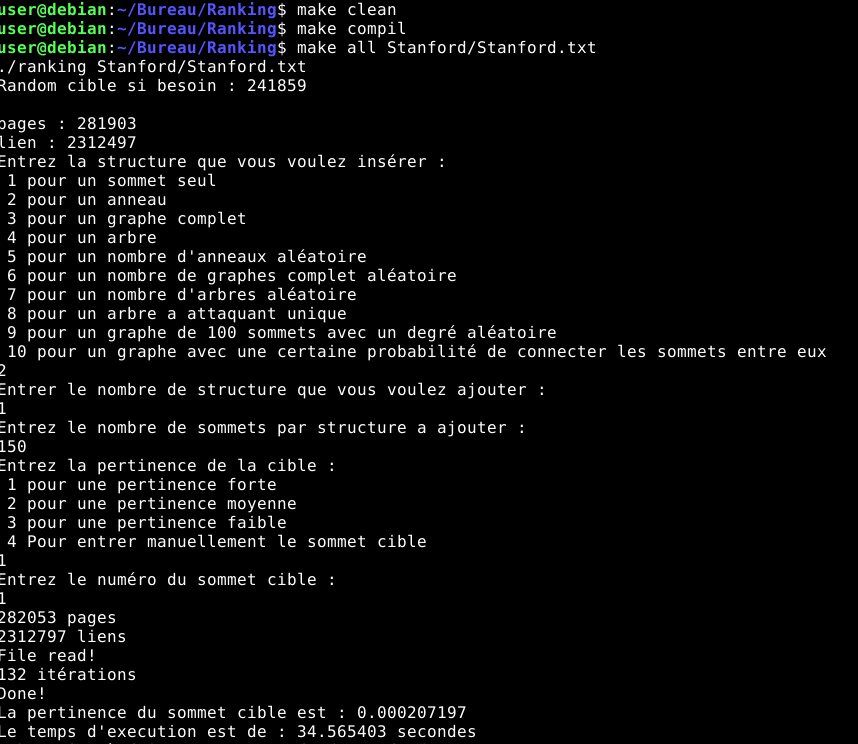
\includegraphics[scale = 0.5]{Captures/manuel.png}\\
	\\
	Dans un premier temps, l'utilisateur doit choisir la structure qu'il veut ajouter au graphe du web qu'il aura préalablement donné.
	Il y a des structures simples (arbre, anneau, graphe complet sommet seuls), des structures moins conventionelles (arbre à attaquant unique, arbre où seul le sommet racine pointe vers la cible). L'utilisateur peut aussi ajouter un nombre de structures aléatoires (avec une limitation de 100 sommets). Il peut également insérer un graphe de degré aléatoire ou un graphe dont le degré est une probabilité.\\
	Dans un deuxième temps,  l'utilisateur doit entrer le nombre de structures qu'il souhaite. Attention, cela ne s'applique pas pour les structures numéro 5, 6 et 7.\\
	Dans un troisième temps, l'utilisateur doit entrer le nombre de sommets de la/les structure(s) à ajouter.\\
	Dans un quatrième temps, l'utilisateur doit entrer le sommet cible. Le numéro du sommet cible est demandé une seconde fois pour savoir quel sommet sera donné en résultat.\\
	\\
	Le programme affiche le nombre de pages, le nombre de liens, le temps d'éxecution et la pertinence du sommet cible.
	
\section{Tests initiaux et hypothèses}
	L'algorithme power calculant les pertinences est contenu dans le fichier \texttt{ranking.c}. Il n'est pas détaillé dans ce rapport mais le fichier est commenté.\\
	\\
	On considère ici le graphe du web Stanford.txt. Ce graphe est modifié par l'ajout de sommets et d'arcs afin d'augmenter la valeur d'un sommet ciblé.\\
	On considère que :\\
	\begin{itemize}
		\item Les sommets représentent les pages du web.
		\item Les arcs représentent les liens dirigeant vers d'autres pages.
		\item Les valeurs des sommets représentent les pertinences calculés par l'algorithme pagerank.
		\item Le sommet cible représente la page dont on souhaite augmenter la pertinence.
		\item 100 sommets sont ajoutés pour chaque test.
	\end{itemize}

	\subsection{Explications du code}
		Les fonctions \texttt{ajoutanneau}, \texttt{ajoutsommetseul}, \texttt{ajoutcomplet} et \texttt{ajoutarbre} crée des structures à la fin du fichier. Ces fonctions ont pour arguments :
		\begin{itemize}
			\item \texttt{nbajout} : le nombre de sommets par structures,
			\item \texttt{nom} : le nom du fichier contenant le graphe du web,
			\item \texttt{nbpages} et \texttt{nbliens} : le nombre de pages et de liens du graphe du web,
			\item \texttt{perticible} : la cible à attaquer,
			\item \texttt{nbstructure} : le nombre de structures à ajouter.
		\end{itemize}
		La fonction \texttt{ajoutanneau} : 
		\begin{lstlisting}
FILE *g = fopen(nom,"a");
for (int y = 0; y < nbstructure; y++) {
	for (i = 1; i < nbajout; i++) {
		fprintf(g, "%d %d %d 0.500000 %d 0.500000\n", 
			nbpages+i+(y*nbajout), degre, 
			nbpages+i+1+(y*nbajout), cible);
	}
	//ecriture du dernier sommet qui se relie au 
	//premier sommet de l'anneau
	fprintf(g, "%d %d %d 0.500000 %d 0.500000\n", 
		nbpages+i+(y*nbajout), degre, 
		nbpages+1+(y*nbajout), cible);
}
	\end{lstlisting}
	Ici $y$ et $i$ vont incrémenter respectivement le nombre de structures et le sommet suivant à écrire. $i$ commence à 1 pour écrire le numéro de la page suivant le dernier numéro de page du graphe.
	Les nouveaux nombres de pages et de liens du graphe sont écrits de cette mainière :
	\begin{lstlisting}
	fprintf(h, "%d %d", nbpages+(nbajout*nbstructure),
	 nbliens+(nbajout*nbstructure)*2);
	\end{lstlisting}
	La fonction \texttt{ajoutcomplet} :
	\begin{lstlisting}
for (int y = 0; y < nbstructure; y++) {
	for (i = 1; i < nbajout + 1; i++) {
		fprintf(g, "%d %d", nbpages+i+(y*nbajout), degre);
		for(j = 1; j < nbajout + 1; j++){
			if (nbpages+j == nbpages+i) {}
			else {
				fprintf(g, " %d %f", 
					nbpages+j+(y*nbajout), x);}
		}
		fprintf(g, " %d %f\n", cible, x);
}	
	\end{lstlisting}
	Le premier \texttt{fprintf} écrit le numéro de la page courante et son degré. Le second \texttt{fprintf} écrit les liens entre cette page et toutes les autres pages du graphe complet. Le \texttt{if} sert à vérifier que l'on écrit pas un lien de la page vers elle-même.\\
	La fonction \texttt{ajoutarbre} :
	\begin{lstlisting}
for (int y = 0; y < nbstructure; y++) {
	// Initialisation du sommet racine
	racine = nbpages + 1+(y*nbajout);
	fprintf(g, "%d %d %d 1.000000\n", racine, 1, cible);
	// Sommets 2 a 2 (arbre binaire) et on pointe 
	//vers le sommet pere 
	// lui meme calcule par sa distance a la racine	
	for (i = 1; i < nbajout - 1; i+=2) {
		fprintf(g, "%d %d %d 0.500000 %d 0.500000\n", 
			racine+i, degre, racine + compteur, cible);	
		fprintf(g, "%d %d %d 0.500000 %d 0.500000\n", 
			racine+i+1, degre, racine + compteur, cible);	
		compteur++;
	}
	// Le dernier sommet dans le cas d'un nombre 
	//PAIR de sommets 
	// a entrer (pair car le sommet racine est deja 
	//ecris hors de la boucle)
	if (nbajout%2 == 0){ 
		fprintf(g, "%d %d %d 0.500000 %d 0.500000\n", 
			racine+i, degre, racine + compteur, cible);
	}
	//on reinitialise le compteur car on va commencer
	//un nouvel arbre
	compteur = 0;
}
	\end{lstlisting}
	\texttt{racine} représente le sommet racine et permet d'écrire les pages suivantes. Les pages sont écrites deux à deux et calculées avec leur distance par rapport à \texttt{racine}. Elles sont écrites deux à deux car on écrit les deux fils d'un sommet père à chaque itération. \texttt{compteur} est utilisé dans le cas de la création de plusieurs arbres.

	\subsection{Résultats des tests initiaux}
		\subsubsection{Stanford.txt sans modification}
			281903 pages\\
			2312497 liens\\
			132 itérations\\
			27.627466 secondes\\
			\\
			Voici les pertinences de base des trois sommets étudiés :\\
			Pertinence forte : Page 280545 - 9.96199e-05\\
			Pertinence moyenne : Page 281466 - 7.53954e-06\\
			Pertinence faible : Page 281574 - 6.05222e-07
		\subsubsection{Résultats}
			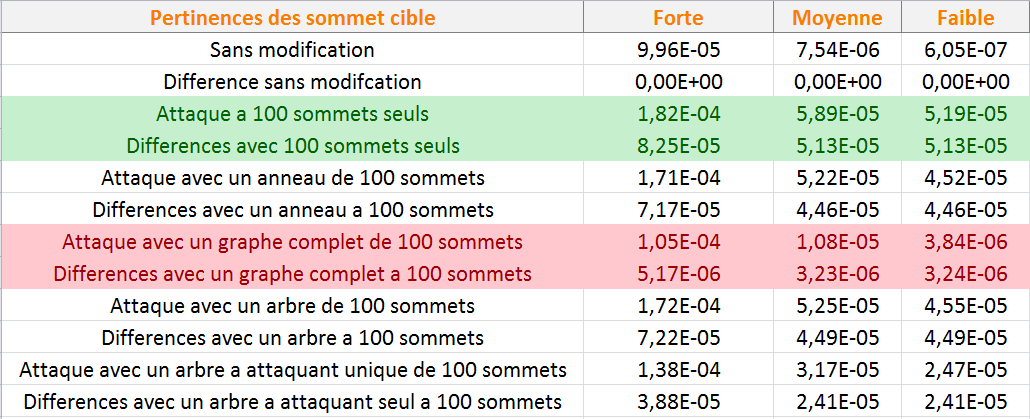
\includegraphics[scale = 0.5]{Captures/ranking1.PNG}

	\subsection{Conclusion des tests initiaux}
		Cinq structures différentes sont ajoutées : des sommets seuls, un graphe complet, un anneau, un arbre et un arbre à attaquant unique(seul le sommet racine est relié à la cible). L'objectif de cette structure est de minimiser le nombre de sommets reliés à la cible pour minimiser les chances de se faire repérer lors de l'attaque.\\
		On observe pour chaque cible que la structure la plus efficace est le sommet seul, suivi de l'arbe, de l'anneau, de l'arbre à attaquant unique et enfin du graphe complet.\\
		La raison de cette ordre serait que pour des sommets seuls, la probabilité de pointer sur la cible est de $1/1$ alors qu'elle est de $1/n$ pour un graphe complet avec $n$ le nombre de sommets. Ainsi la probabilité est dilué et donc la cible en sera moins modifié.\\
		On observe que pour chaque structure la différence de modification de la pertinence est presque identique entre les cibles faibles et moyennes.
		Ainsi on peut en déduire que modifier la pertinence d'une cible à $10^{-06}$ ou $10^{-05}$ est de même difficulté.\\		
		Pour le sommet seul, on observe que la modification de pertinence (la différence) pour une cible forte, moyenne ou faible sont respectivements $8,25.10^{-05}$, $5.13.10^{-05}$ et $5,13.10^{-05}$. On peut donc en déduire que modifier la pertinence d'une cible est plus significative quand la cible est déjà à pertinence forte.
			
	\subsection{Hypothèses}
		On suppose que les structures les plus efficaces sont les sommets seuls et les arbres. On suppose que changer la pertinence d'une cible devient 
		plus difficile à partir d'une cible de pertinence $X.10^{-05}$ et que c'est assez identique pour les cibles de pertinences $X.10^{-06}$ et $X.10^{-07}$.


\section{Tests avec un nombre de graphes générés aléatoirement}
	Nous allons désormais insérer des graphes générés aléatoirement. Ce qui est aléatoire n'est pas la structure des graphes mais le nombre de garphes générés.\\
	L'objectif de cette démarche est de déterminer quel structure est la plus efficace globalement, c'est-à-dire quelle structure influe le plus sur la pertinence quelle que soit la situation.\\
	De plus, les résultats nous aiderons aussi à déterminer l'impact qu'à une certaine structure sur la cible de manière plus générale que dans les cas prédéfinis de la partie précedente.
	Le nombre de sommet des graphes ajoutés est fixé à $100$.
	La cible est également fixée ainsi que la structure des graphes ajoutés.\\
	Par exemple, 5 graphes complets de nombre de sommet sont insérés, respectivement : 25, 10, 5, 6 et 4. Tous sont reliés au sommet cible.\\
	Tout d'abord, le code derrière cette démarche.
	Puis, l'analyse des résultats.

	\subsection{Explication du code}
		Tous est dans le fichier \texttt{ajoutsommetsattanquants.c}. Les fonctions utilisées sont \texttt{ajoutanneaualeatoire}, \texttt{ajoutcompletaleatoire}
		et \texttt{ajoutarbrealeatoire}. Ces fonctions reprennent en partie le code des trois fonctions presque éponyme décrites précedemment.
		Regardons ce qui a changé :
		\begin{lstlisting}
while(nbsommetrestant > 0) {
	nbajout = rand()%(100-nouveausommets);
	if (nbajout <= 3) { nbajout = 3; }
	nbsommetrestant -= nbajout;
		\end{lstlisting}
		\texttt{nbajout} représente le nombre de sommets que l'on ajoute dans la première structure créée. Il récupère un nombre aléatoire compris entre $0$ et $100$ car le nombre de sommets total est limité a $100$. Si le nombre obtenu est inférieur à $3$ on le fixe à $3$ car créer des anneaux ou des graphes complets de tailles inférieure à $3$ revient à créer des sommets seuls. \texttt{nbajout} est enlevé au nombre de sommets à ajouter. Puis, on lance la construction de la structure comme vu précedemment avec \texttt{nbajout} représentant le nombre de sommets. A la fin de cette itération \texttt{nbajout} reprend un nombre aléatoire qui compris entre $0$ et $100$ moins le nombre de sommets ajoutés précédement représenté par \texttt{nouveausommets}.

	\subsection{Résultats des tests}
		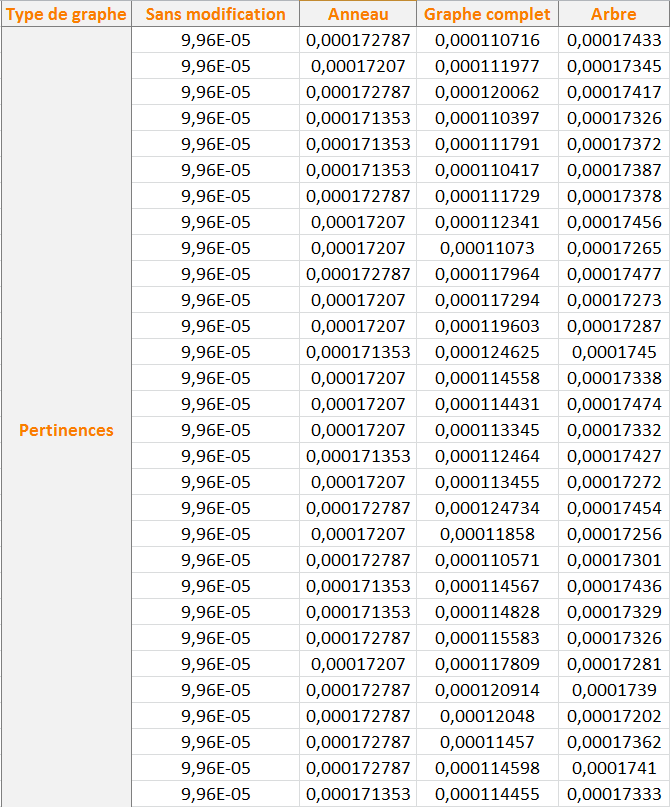
\includegraphics[scale = 0.5]{Captures/ranking2.PNG}\\
		La cible est de pertinence forte. \\
		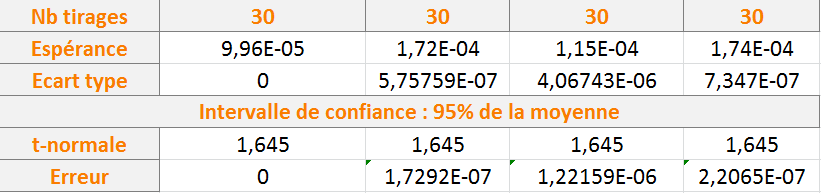
\includegraphics[scale = 0.5]{Captures/ranking3.PNG}\\
		En regardant les espérances, nous pouvons observer que l'anneau et l'arbre impactent le plus la pertinence de la cible. Nous observons aussi que les erreurs sont inférerieurs à $1,5*10^{-5}$. On peut donc faire confiance aux résultats.\\
		\\
		Regardons les trois courbes en annexe.\\
		"Quoi qui où ??? Num page ? Nom/num annexe"\\
		\\
		La courbe rouge représente la loi normale, la noire est la fonction de densité.\\ 
		Comparons ces résultats avec les résultats des tests initiaux. Les résultats sont comparables car dans les deux cas $100$ sommets sont ajoutés. Dans les tests initiaux les pertinences après attaque pour l'anneau, le graphe complet et l'arbre étaient respectivement $1,71.10^{-4}$, $1,05.10^{-4}$ et $1,72.10^{-4}$. On remarque donc qu'il n'y a que $0,6$\% de différence pour l'anneau et $1,1$\% pour l'arbre. En revanche, pour le graphe complet il y a $9.5$\% de différence ce qui est bien plus intéressant.

	\subsection{Conclusion sur l'impact d'un nombre aléatoires de structures}
		Créer plusieurs structures pour attaquer la cible n'est pas efficace pour les structures de l'anneau et de l'arbre. Cependant, la structure du graphe complet est plus efficace si on en crée plusieurs. 

\section{Expériences avec un graphe de degré aléatoire}
	Nous allons créer un graphe de $100$ sommets de degré aléatoire. C'est-à-dire que chaque sommet sera relié au même nombre de sommets au sein du graphe.\\
	\\
	"??? Bah non aléatoire ça veut pas dire que c'est le même nombre de sommet"

	\subsection{Résultats des tests}
		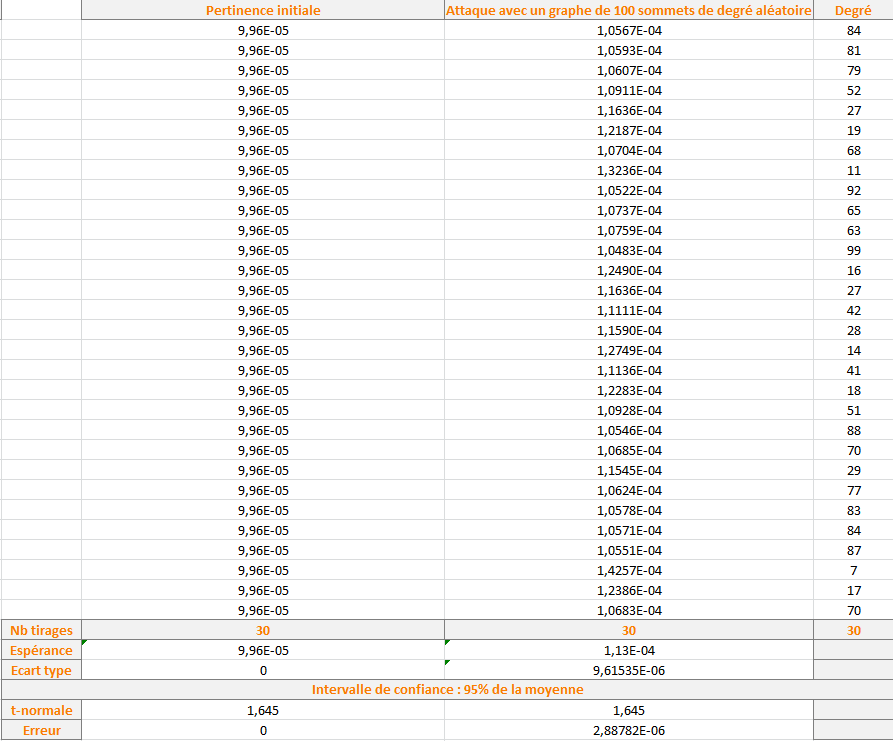
\includegraphics[scale = 0.5]{Captures/ranking4.PNG}\\
		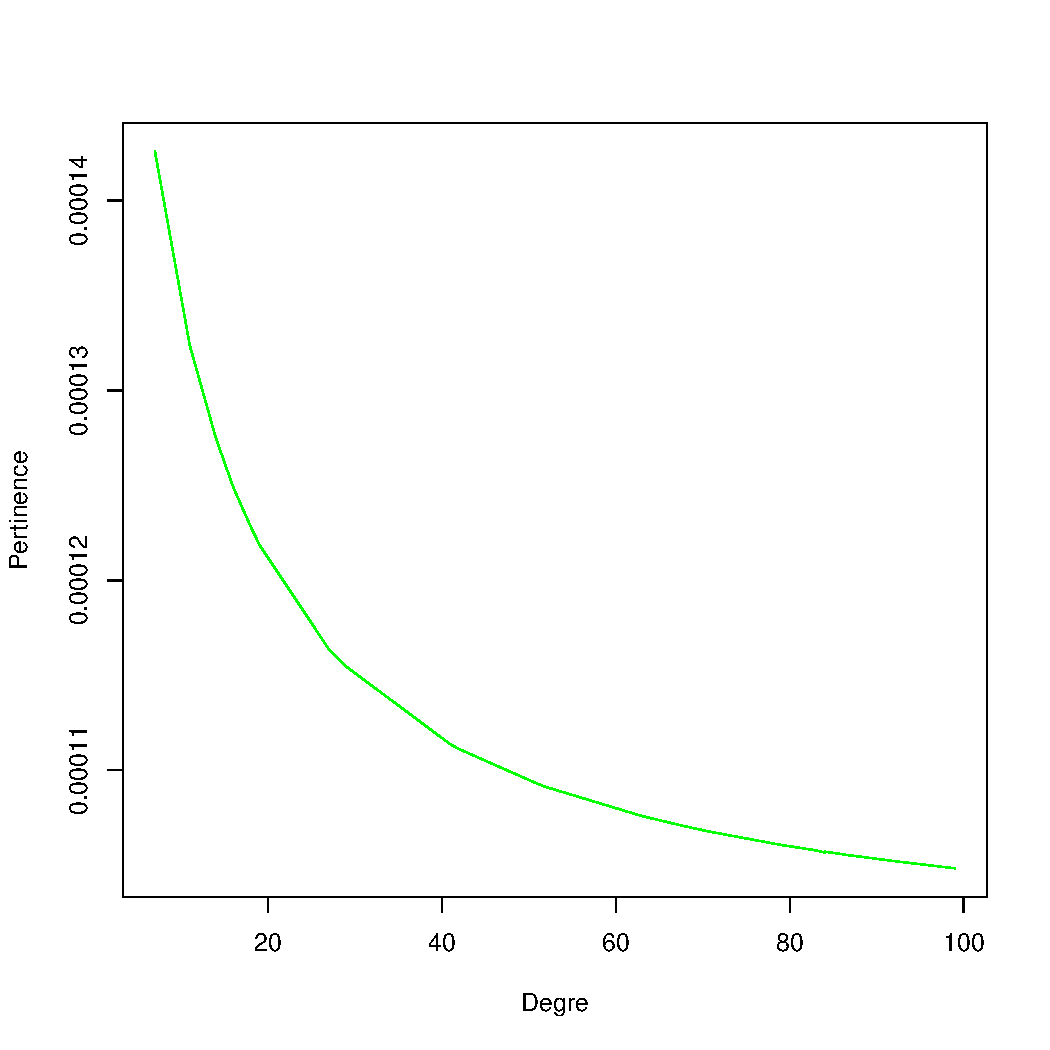
\includepdf{../R/Degre_aleatoire/degre.pdf}
	
	\subsection{Analyses}
		On observe sur le graphique que plus le degré est fort, moins la pertinence de la cible est impacté. L'espérance de la pertinence de la cible après attaque est de $1,13.10^{-4}$, ce qui est meilleur que la pertience de la cible lors des tests initiaux avec un graphe complet à $100$ sommets ($1,05.10^{-4}$). Donc, cette structure est plus efficace que le graphe complet. De plus, cette structure a l'avantage d'être moins "détectable" que l'anneau ou le graphe complet car le degré varie.
	

\section{Expériences sur l'efficacité}
	
	\subsection{Résultats des tests}
		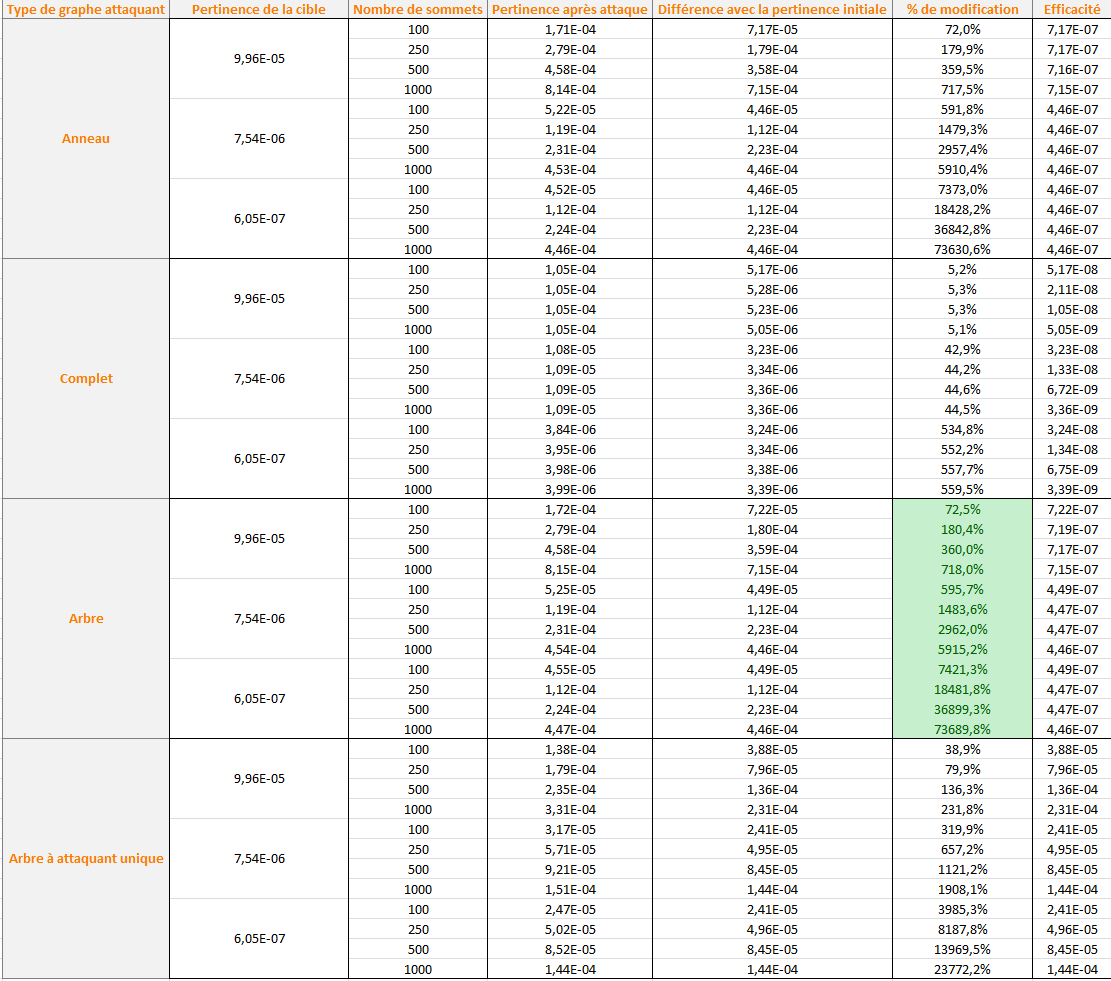
\includegraphics[scale = 0.5]{Captures/ranking5.PNG}\\
		Nous avons testé chaque structure sur trois cibles différentes, tout en faisant varier le nombre de sommets par structure. 
		Le pourcentage de modification est calculé. L'efficacité est calculé en divisant la différence par rapport à la pertinence initiale par le nombre de sommets ajoutés.
	\subsection{Analyses}
		On observe que, toutes pertinences confondues, la structure qui modifie le plus la cible est l'arbre, suivie de l'anneau, de l'arbre à attaquant unique et enfin du graphe complet. Cela confirme nos hypothèses des tests initiaux. La raison de cette efficacité est que la pertinence ne se disperse que très peu dans ces structures, ce qui permet d'attaquer la cible efficacement. Par exemple, dans un anneau chaque sommet reçoit la pertinence d'un de ses voisins puis pointe sur la cible. Ainsi la pertinence est équitablement répartie et peu dispersée au sein de la structure.\\
		Pour l'arbre on observe un phénomène similaire car chaque sommet est relié à son sommet père et à la cible. On peut expliquer la légère différence entre arbre et anneau par le fait que plus on monte dans l'arbre, plus la pertinence est forte. Ainsi les attaques des sommets les plus hauts dans l'arbre sont plus efficaces sur la cible.\\
		\\
		On observe que, pour toutes structures confondues, la différence avec la pertinence initiale est quasiment identique entre une cible moyenne ($7,5.10^{-6}$) et faible ($6,05.10^{-7}$), c'est-à-dire qu'on modifie autant la cible qu'elle soit de pertinence moyenne ou faible.\\
		Nous pouvons en conclure que les cibles en dessous de $X.10^{-6}$ sont toutes très similaires à attaquer.\\
		\\
		Pour l'anneau, le graphe complet et l'arbre on observe que la différence avec la pertinence initiale augmente de manière linéaire avec l'augmentation du nombre de sommets.\\
		Par exemple, pour l'arbre attaquant une cible à pertinence forte, on passe de $7,22.10^{-5}$, $1,80.10^{-4}$, $3,59.10^{-4}$, $7,15.10^{-4}$ pour $100$, $250$, $500$ et $1000$ sommets. Ce qui est presque linéaire. Ce phénomène arrive quelque soit la pertinence de la cible.\\
		Donc, nous pouvons en conclure que pour obtenir une attaque la plus efficace possible il faut augmenter le nombre de sommets au maximum. Cependant, plus il y a de sommets, plus il est facile de "détecter" une attaque. Une stratégie raisonable serait d'utiliser un arbre de $500$ sommets, ce qui modifie la pertinence de la cible de $360$\% tout en ne représentant que $0,18$\% du graphe du web. De plus, une structure en arbre peut être difficile à reconnaitre si l'attaquant décide de modifier légèrement sa structure. Par exemple, enlever certains liens pointant vers la cible peuvent donner cela : \\
		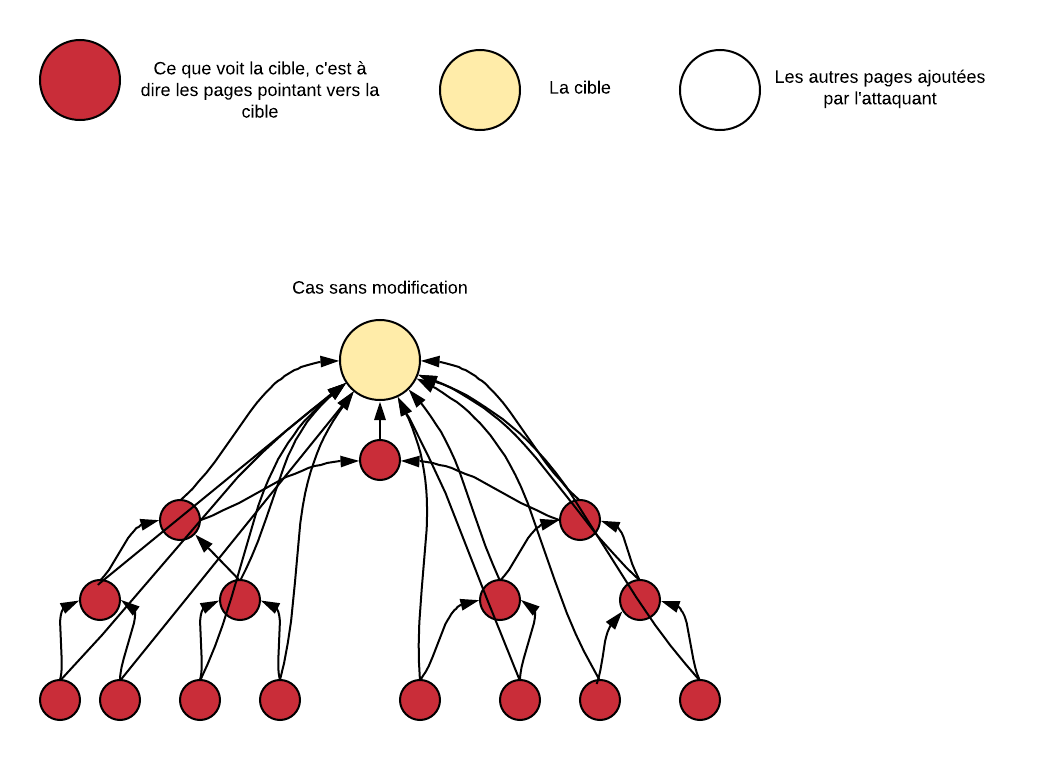
\includegraphics[scale = 0.5]{Captures/diagramme1.png}\\
		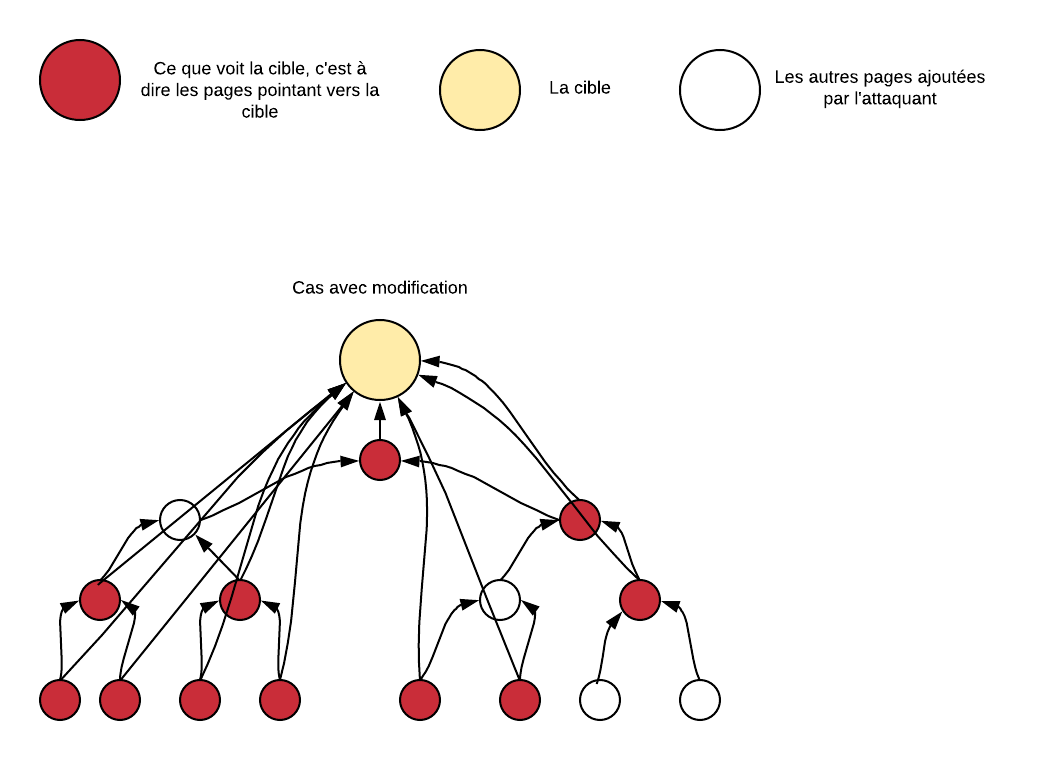
\includegraphics[scale = 0.5]{Captures/diagramme2.png}\\
		La cible ne peut détecter que les pages qui pointent directement sur elle, c'est-à-dire les sommets en rouge.\\
		La seconde structure est légèrement moins efficace mais elle rend plus difficile la détection de l'attaque. En effet, les sommets ne sont plus reliés ensemble en forme d'arbre du "point de vue" de la cible.\\
		C'est donc une stratégie possible.\\
		\\
		Nous observons que les valeurs d'efficacité les plus grandes sont pour l'arbre à attaquant unique. Cela s'explique par le fait que un seul sommet est relié à la cible dans cette structure. Néanmois, les pourcentages de modifications sont bien plus faible que pour l'arbre ($38$\% contre $72$\% pour une cible à pertinence forte à $100$ sommets attaquant).\\
		Mais cette structure reste très utile pour des cibles moyennes ou faible. Ainsi une startégie intéressante pour les cibles faibles serait d'utiliser un arbre à attaquant unique. Son avantage majeur est qu'il est tres difficil à détecter car un seul sommet est directement relié à la cible.
	
\section{Conclusions}
	Tout d'abord, nous avons pu constater que nos hypothèses initiales sont vérifiées. La pertinence de la cible devient signifactive à partir de $X.10^{-5}$, et l'arbre est la structure la plus efficace. Nous avons remarqué qu'utiliser plusieurs structures n'améliore pas l'efficacité du changement de pertinence. Un graphe de degré aléatoire est plus efficace qu'un graphe complet mais moins qu'un anneau, l'intérêt de cette structure est donc d'améliorer la discrétion de l'attaque.\\
	Finalement, nous concluons que l'abre est le plus efficace quelque soit le nombre de sommets attaquant et quelque soit la cible (pertinence forte, moyenne ou faible). De plus des structures alternatives à l'arbre peuvent aider à rendre l'attaque encore plus discrète.\\
	\\
	La structure de l'arbre est donc la plus efficace, particulièrement pour les cibles fortes.\\
	Pour les cibles moyennes et faibles, un arbre à attaquant unique (seul le sommet racine pointe vers la cible) est un choix judicieux car il est très dur à détecter et améliore de manière notable la pertinence pour ces types de cibles.

\section{Annexe}
	Annexe 1 :\\
	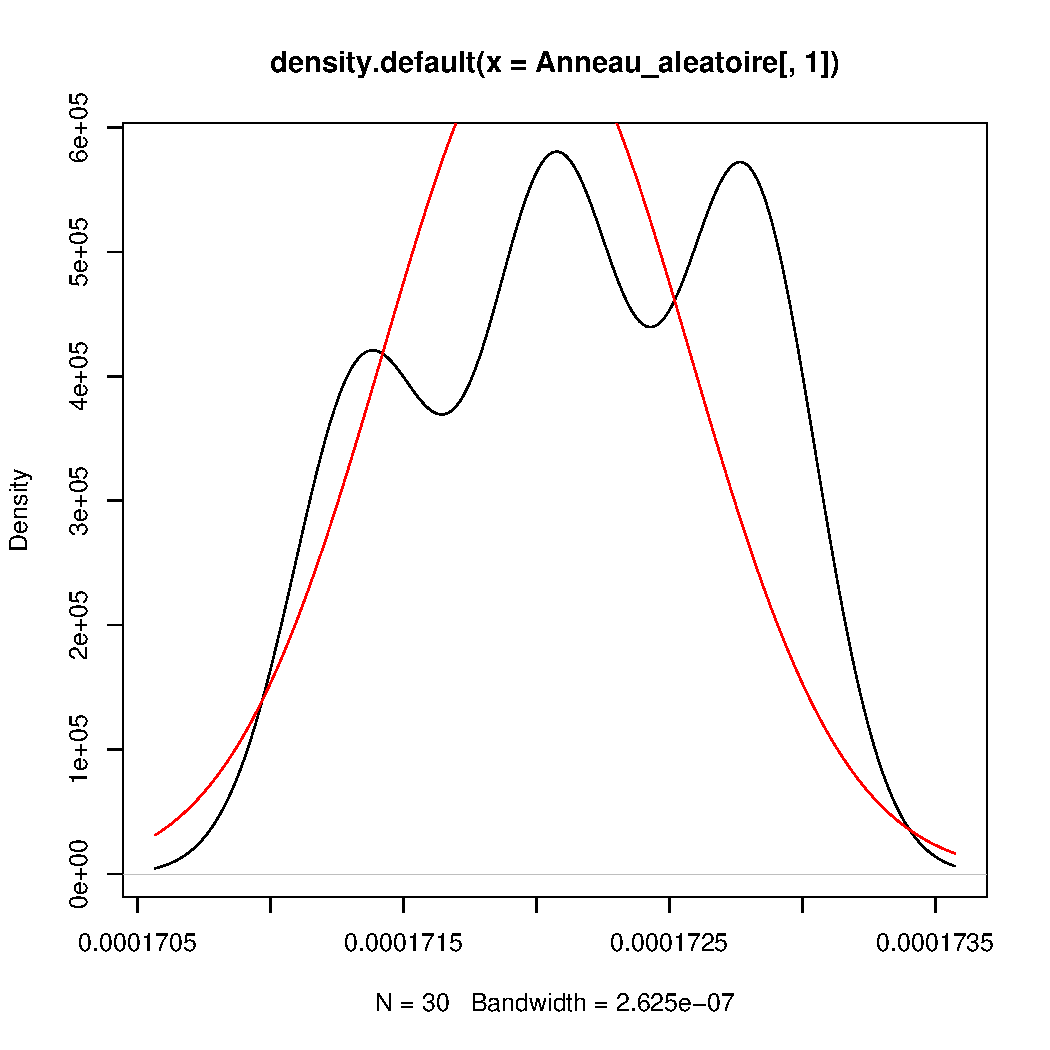
\includepdf{../R/Nombre_de_graphe_aleatoire/Anneau.pdf}

	Annexe 2 :\\
	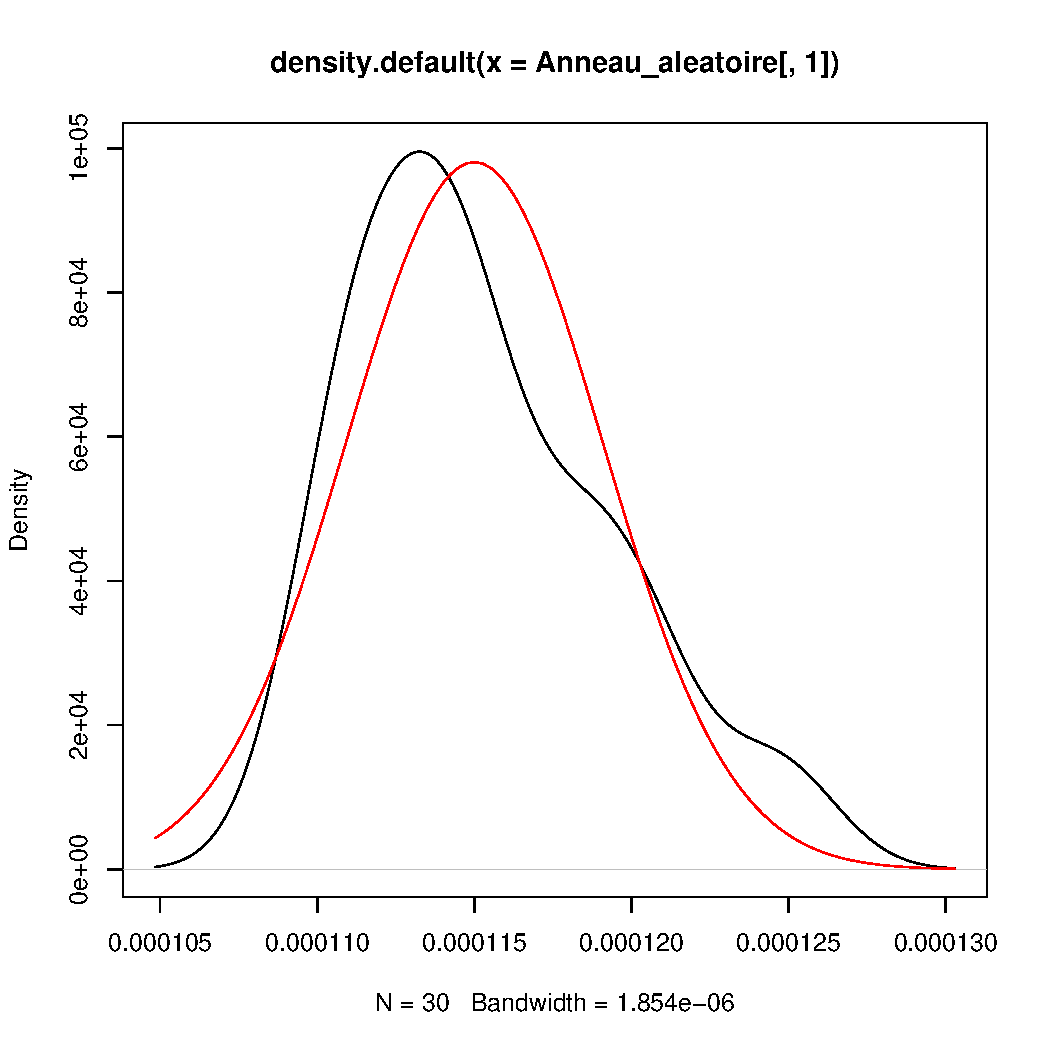
\includepdf{../R/Nombre_de_graphe_aleatoire/Complet.pdf}

	Annexe 3 :\\
	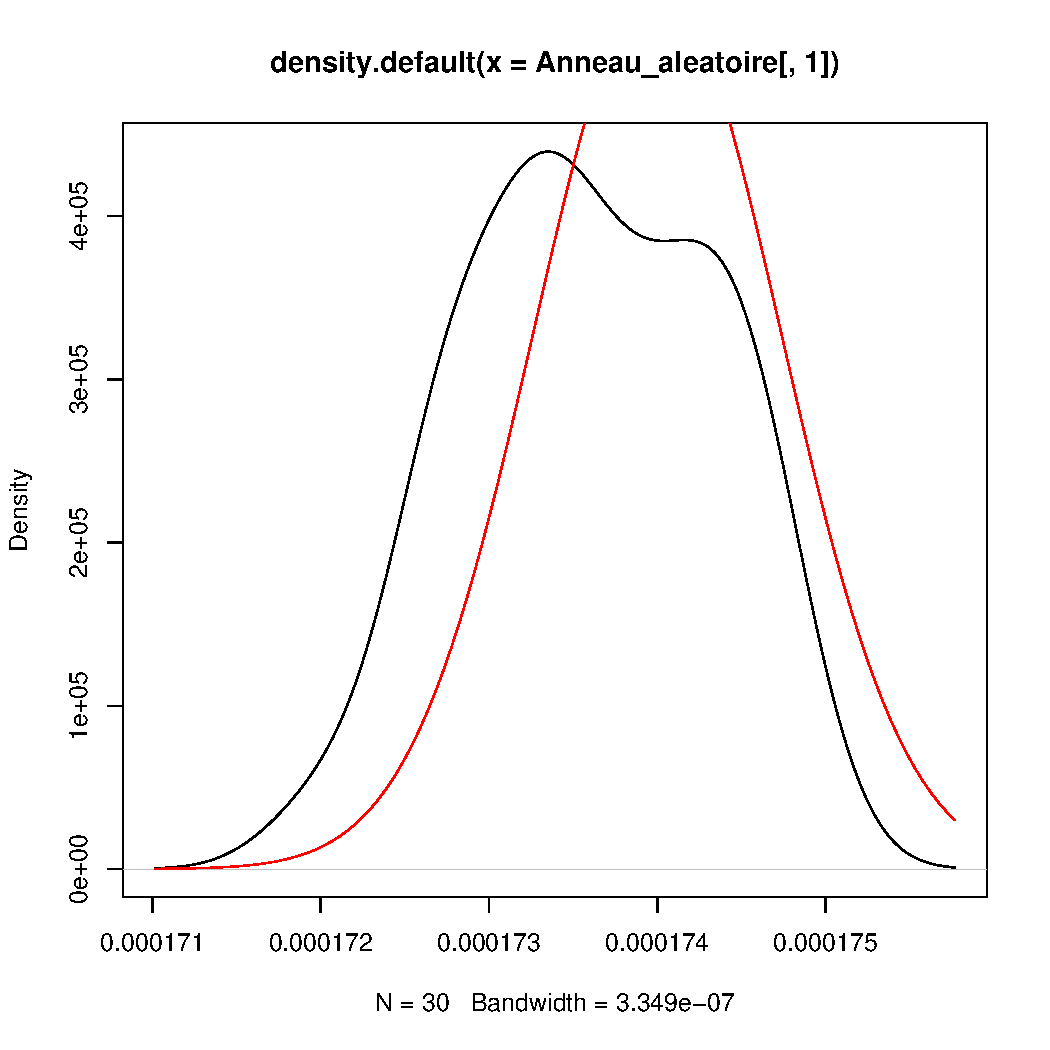
\includepdf{../R/Nombre_de_graphe_aleatoire/Arbre.pdf}

\end{document}
